        \documentclass{standalone}
        \usepackage{tikz}
        \usetikzlibrary{arrows}
        \usepackage{amsmath}
        \usepackage{amsfonts}
        \begin{document}
        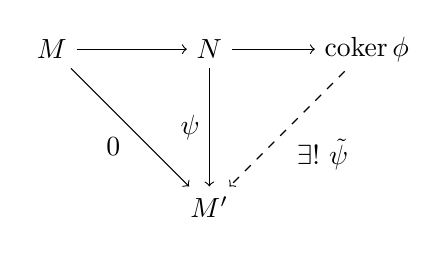
\begin{tikzpicture}

    \node (T) at (0,-2) {$M^\prime$};
    \node (M) at (-2,0) {$M$};
    \node (N) at (0,0) {$N$};
    \node (coker) at (2,0) {$\operatorname{coker} \phi$};
    \draw[->] (N) -- node[left] {$\psi$} (T);
    \draw[->] (M) -- node[below left] {$0$} (T);
    \draw[->,dashed] (coker) -- node[below right] {$\exists ! ~\tilde{\psi}$} (T);
    \draw[->] (N) -- (coker);
    \draw[->] (M) -- (N);
        \end{tikzpicture}
        \end{document}
